\documentclass{memoir}
\usepackage{geometry, hyperref, listings, xcolor, graphicx}

\title{Project of Distributed Systems: Blockchain Inventory System}

\author{Cancian Matteo and Del Pio Luogo Marco}

\date{Version 0.2, \today}

\begin{document}

\maketitle
\begin{abstract}
...
\end{abstract}

\chapter{Chapter 1}\label{ch:intro}
In this chapter you describe the main problem, and an idea of the solution.
It is not necessary to be very detailed or formal, but it is important to explain which are the main aims and issues from the point of view of Distributed Systems:
\begin{itemize}
\item A description of the application.
\item The overall structure of the implementation: how resources are deployed, which are the players, the r\^oles.
\item The distributed system features (and the transparencies) and algorithms you intend to implement.
\item Your plan for testing the system.
\item A schedule for how you plan to carry our your design and implementation
\end{itemize}

\section{Introduction}

Il presente progetto si propone di sviluppare un sistema distribuito dedicato alla rendicontazione di asset ed elementi d'inventario in contesti dove è fondamentale garantire sicurezza, trasparenza, integrità e ordine cronologico delle operazioni registrate.
Il sistema quindi sarà usato dagli operatori aziendali per la tracciabilità delle dei movimenti riguardanti qualsiasi oggetto interno all'azienda per la gestione dell'inventario. 
Tale sistema dovrebbe essere capace di eseguire le operazioni di 'inbound' e 'outbound', permettendo così di registrare quando una merce entra ed esce definitivamente dall'inventario. 
Il sistema dovrebbe essere capace anche di gestire gli errori da parte degli operatori umani (o non umani), permettendo di correggerli/rimediare. 

Il sistema deve avere un metodo di accesso e uso intuitivo per l'operatore, fornendo le indicazioni giuste per eseguire le operazioni menzionate prima (inclusa la correzione di operazioni). 
Si pretende che il sistema sia usato in una azienda dove l'inventario sia condiviso tra tanti sedi a livello nazionale/continentale, portando quindi problemi riguardanti alla decentralizzazione delle informazioni contenute nel sistema e alla gestione di esse, oltre che . 
Per le informazioni riguardanti l'inventario aziendale quindi si richiede l'\textit{integrità} e l'\textit{accountability} alle modifiche di tali informazioni.

Per soddisfare questi rigorosi requisiti, si prevede di implementare un sistema distribuito con i seguenti nodi: 

\begin{itemize}
    \item \textbf{Nodo blockchain:} È responsabile dell'aggiornamento e salvataggio della blockchain contenente tutti i dati relativi alle operazioni dell'inventario. 
    Questo nodo è anche responsabile dell'esecuzione di algoritmi che permettano la gestione della \textit{concorrenza}, il \textit{consenso distribuito}  

    \item \textbf{Nodo client:}
\end{itemize}


. In tale architettura si integra la tecnologia blockchain applicandola direttamente ai log delle transazioni, 
offrendo così una soluzione ottimale per garantire l'immutabilità della sequenza storica, l'affidabilità del dato e la piena accountability.

\subsection{Vantaggi della blockchain}

La blockchain risponde, a molti dei problemi storici legati alla rendicontazione di asset e proprietà, come ad esempio:

Immutabilità e lotta alle frodi: In un database tradizionale, un amministratore di sistema corrotto (o un hacker) potrebbe alterare quantità o altre proprietà di un oggetto d'inventario, falsificando lo storico. 
Sulla blockchain, una volta che un blocco di dati è consolidato, modificarlo retroattivamente è praticamente quasi impossibile.

Tracciabilità storica perfetta: La natura stessa della blockchain crea una catena ininterrotta. 
Questo permetterebbe di risalire a tutti i precedenti movimenti dell'oggetto in modo istantaneo e inequivocabile, eliminando dispute legali.

Automazione tramite Smart Contract: Si potrebbero creare "contratti intelligenti" che eseguono automaticamente il passaggio di proprietà solo quando i 
fondi vengono effettivamente trasferiti. Questo ridurrebbe drasticamente i tempi di attesa e, potenzialmente, i costi di intermediazione (come quelli notarili).

Resilienza dell'infrastruttura: Essendo un registro distribuito su migliaia di nodi (computer) indipendenti, 
la blockchain non ha un "singolo punto di fallimento". È immune alla distruzione fisica dei server centrali a causa di incendi, guerre o disastri naturali.

\subsection{Svantaggi della blockchain}

Problema "Garbage In, Garbage Out": La blockchain garantisce che i dati non vengano manomessi dopo essere stati inseriti, 
ma non può verificare se il dato iniziale sia vero. Se un truffatore riesce a registra un movimento falso di un oggetto, 
la blockchain renderà semplicemente quella menzogna "immutabile". La necessità di un'autorità rimane fondamentale.

Efficienza tecnica: I database relazionali tradizionali sono infinitamente più veloci, economici e facili da 
aggiornare rispetto a un'infrastruttura blockchain.

Gestione degli errori: Se in un catasto tradizionale viene fatto un errore di battitura, un funzionario autorizzato lo corregge. 
Sulla blockchain, modificare un errore richiede procedure molto più complesse, poiché l'architettura è progettata proprio per impedire le modifiche.





-----------------------------------------------------------------------------------------------------------------------

Se i nodi che validano le transazioni sono entità note, autorizzate e pre-approvate, non siamo più nel mondo delle blockchain "pubbliche" come Bitcoin, e non si usano algoritmi dispendiosi come la Proof of Work.

Questa architettura si definisce Blockchain Permissioned (o di Consorzio). L'algoritmo di consenso più utilizzato in questi casi si chiama Proof of Authority (PoA).

Come funziona la Proof of Authority: Non c'è "mining" e non si mettono in gioco criptovalute. Il diritto di generare un nuovo blocco valido
è affidato ad una maggioranza di nodi che hanno dimostrato la loro identità (i server di enti governativi o notarili). 
Il consenso viene raggiunto perché i nodi si fidano dell'identità crittografica degli altri nodi. 
Se un nodo "impazzisce" o viene hackerato, gli altri server della rete lo escludono. 
Altri algoritmi simili usati in questi contesti sono basati su protocolli BFT (Byzantine Fault Tolerance).







\chapter{Analysis}\label{ch:analysis}

In this chapter, we describe in detail functional and non-functional requirements of a solution for the problem.

\section{Functional requirements}
Which functions must be offered to users / other programs?  Which are the input data and the output data? Which is the expected effect? 

\section{Non functional requirements}
Everything about mode and transparencies: availability, mobility, security, fault tolerance, etc.

Are there execution time bounds? Minimum data rates?

If requested, specific platforms/languages/middlewares requirements for the implementation can be decided here. (E.g.: if the project is on a SOA, we may request that functions are offered via SOAP or RESTful services). 



\chapter{Project}

This chapter is devoted to the description of the general architectures, and specific algorithms.

\section{Logical architecture}
Describe the components of your systems: modules/objects/components/services.
For each component, describe the functionalities it implements, and by who is used.
Modello logico
\begin{figure}[htbp]
    \centering
    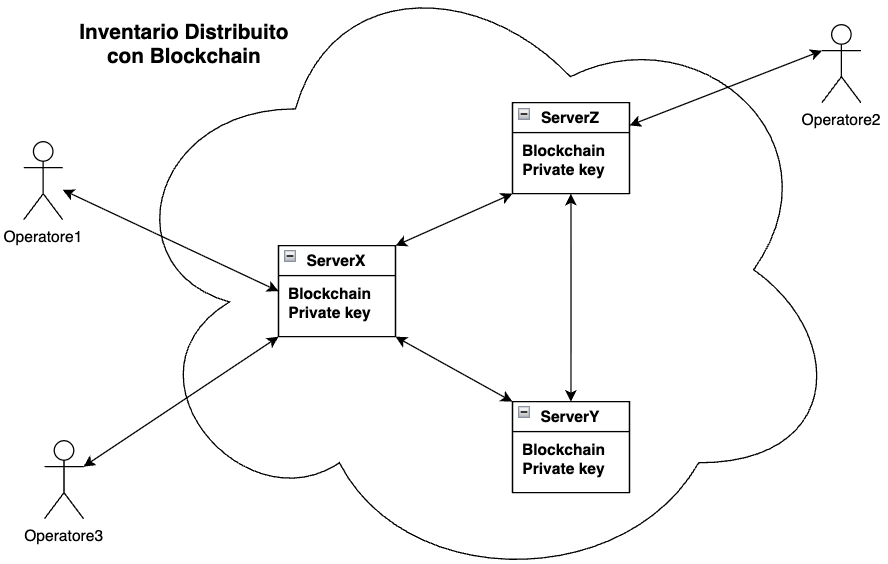
\includegraphics[width=0.7\textwidth]{UML_architettura.png}
    \label{fig:uml_architecture}
\end{figure}
Network behaviour: FAIR-LOSS; Messages can be lost, duplicated, or reordered. If one keeps retrying, a message eventually gets through.
Node behaviour: Adversarial; A node may deviate from the specified algorithm and do anything, including crashing or any malicious action (blocking of messages, replaying, forging, ...).
Timing behaviour: Synchronous; message latency no greater than a known bound; nodes execute algorithm at a known minimum speed; clock drift (i.e. difference between clock speeds at two nodes) within a known range.

\section{Protocols and algorithms}
Communication between components.  UML sequence diagrams go here.
Also, put here a detailed description of distributed algorithms used to solve specific problems of the project.
\begin{figure}[h]
  \centering
  \subfloat[Diagramma attività 1]{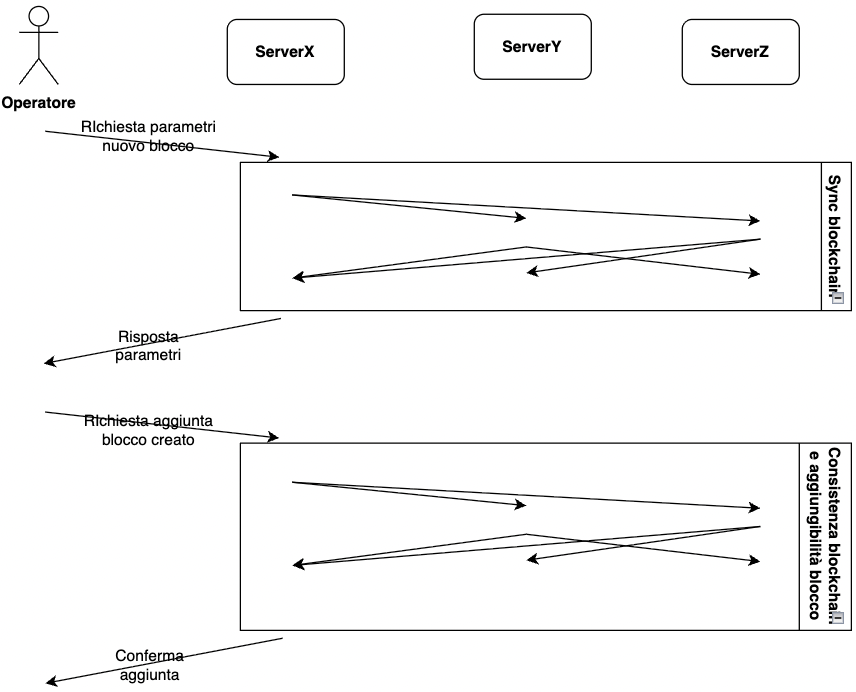
\includegraphics[width=0.45\textwidth]{UML_attivita.png}}
    \label{fig:uml_activity1}
  \hfill
  \subfloat[Diagramma attività 2]{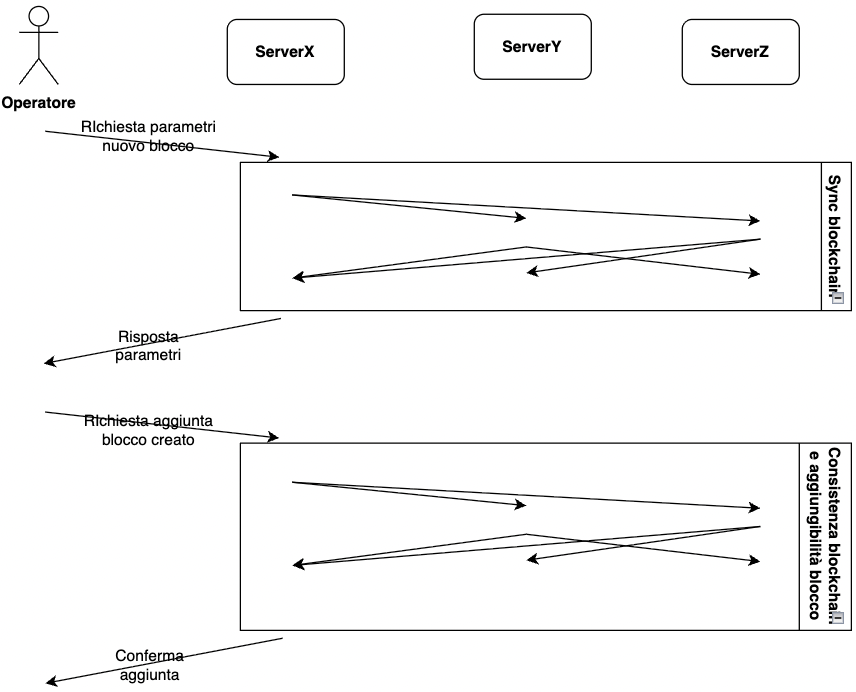
\includegraphics[width=0.45\textwidth]{UML_attivita.png}}
    \label{fig:uml_activity2}
\end{figure}

\section{Physical architecture and deployment}
Which nodes and platforms involved, and where each component is deployed.

\section{Development plan}
Since it is difficult to predict just how hard implementing a new system will be, you should formulate as a set of ``tiers,'' where the basic tier is something you’re sure you can complete, and the additional tiers add more features, at both the application and the system level.


\chapter{Implementation}

Details about the implementation: every choice about platforms, languages, software/hardware, middlewares, which has not been decided in the requirements.


Important choices about implementation should be described here; e.g., peculiar data structures.


\chapter{Validation}

Check if requirements from Chapter~\ref{ch:analysis} have been fulfilled.
Quantitative tests (simulations) and screenshots of the interfaces are put here.


\chapter{Conclusions}

What has been done with respect to what has been promised in Chapters~\ref{ch:intro} and \ref{ch:analysis}, and what is left out.

\appendix

\chapter{Appendix}

In the Appendix you can put code snippets, snapshots, installation instructions, etc.


\chapter*{Evaluation}
Your system will be judged mainly on how it operates as a distributed system. The primary evaluation will be according to whether your system has the following attributes:
\begin{itemize}
\item  It should be an interesting distributed system, making use of some of the algorithms we have covered in class for distributed synchronization, replication, fault tolerance and recovery, security, etc.
\item The software should be well designed and well implemented, in terms of the overall architecture and the detailed realization.
\item You should devise and apply systematic testing procedures, at both the unit and systems levels.
\item The system should operate reliably and with good performance, even in the face of failures.
\end{itemize}
Important, but secondary considerations include:
\begin{itemize}
\item Time taken to do the project (the sooner the better, but do not miss details in order to end sooner)
\item  How nice is the application's appearance: does it have a nice interface or a compelling visual display?
\end{itemize}

\end{document}